\chapter{Methodology}

\section{Overview}

Figure~\ref{fig:pipeline} shows the system. A question goes to a retriever, which picks one passage out of a library of 3,000 Bangla Wikipedia passages. The question and that passage are then given together to the fine-tuned BanglaT5 model, which writes the answer. The model is trained once. After that it is used unchanged with every retriever, so any difference between two conditions comes from the passage it was given.

\begin{figure}[H]
	\centering
	\IfFileExists{figures/pipeline.png}{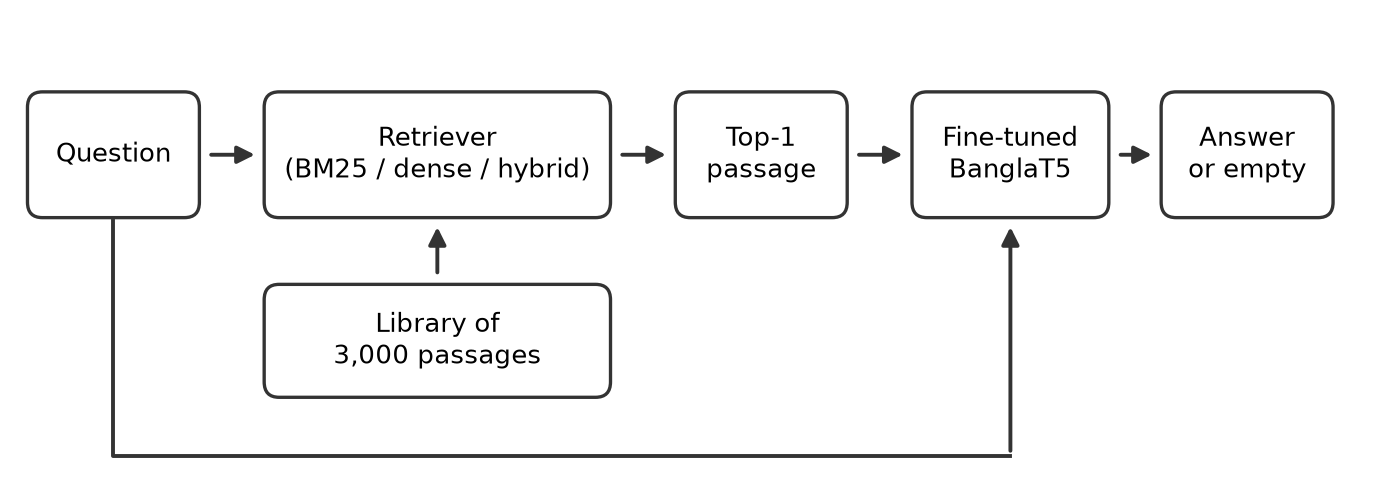
\includegraphics[width=\textwidth]{figures/pipeline.png}}{\todo{figures/pipeline.png is missing; run make\_figures.py}}
	\caption{The question-answering pipeline. The question is used twice: to search the library and as part of the input to the reader.}
	\label{fig:pipeline}
\end{figure}

\section{Dataset}

\subsection{BanglaRQA}

The system uses BanglaRQA \cite{ekram2022banglarqa}, which is released under the CC BY-NC-SA 4.0 licence. The data is downloaded when the code runs and is not shipped with it. Each of the 3,000 Wikipedia passages comes with several questions. A question has a type (factoid, causal, confirmation or list), a flag that says whether the passage answers it, and one or two reference answers. An answer is a single span, several spans separated by semicolons, or a yes/no word.

The official split is used as it is (Table~\ref{tab:split}). It is made by passage, so no passage appears in two splits. About a quarter of the questions in every split cannot be answered from their passage.

\begin{table}[H]
	\centering
	\caption{BanglaRQA splits used in this project.}
	\label{tab:split}
	\begin{tabular}{lrrr}
		\toprule
		Split & Passages & Questions & Unanswerable \\
		\midrule
		Train & 2,400 & 11,912 & 2,904 (24.4\%) \\
		Validation & 300 & 1,484 & 358 (24.1\%) \\
		Test & 300 & 1,493 & 369 (24.7\%) \\
		\bottomrule
	\end{tabular}
\end{table}

Five question ids are used twice in the test split. They belong to one passage, about the becquerel, which has ten questions attached; five of them are about the Shah Amanat Bridge and cannot be answered from that passage's text. Because of this, retrieval results are stored under the id together with the question text, and these five questions are left in the test set. They are 0.3\% of the questions.

\subsection{Preprocessing}

Question, passage and answer are all normalised with the \texttt{normalizer} package from the BanglaT5 authors, as its documentation requires. The training target is the first reference answer. For an unanswerable question the target is the empty string. If a question has two reference answers, only the first is used for training and for scoring, which is what the dataset authors do.

For the BanglaT5 tokenizer the median input (question plus passage) is 293 tokens. The input limit is 1,024 tokens, and 10 of the 11,912 training inputs reach it and are cut.

\section{The Reader: Fine-Tuned BanglaT5}

\subsection{Model}

The reader is BanglaT5 (\texttt{csebuetnlp/banglat5}) \cite{bhattacharjee2023banglat5}, an encoder-decoder Transformer with 12 layers in each half and about 247 million parameters, built on the T5 design \cite{raffel2020t5}. The encoder reads the question and the passage together and the decoder writes the answer one token at a time.

\subsection{Input and Output Format}

The tokenizer receives the question and the passage as a pair, question first. If the pair is longer than 1,024 tokens the passage is cut, never the question. The target is the normalised first reference answer, at most 256 tokens. An unanswerable question has an empty target, so the model learns to write nothing when the passage has no answer. This follows the dataset authors' published training code \cite{ekram2022banglarqa}.

\subsection{Training}

Training minimises the usual cross-entropy loss over the answer tokens. Examples of similar length are batched together so that short inputs are not padded up to the length of long ones. Weights are kept in 32-bit precision and the forward pass runs in bfloat16, because T5 models are known to overflow in 16-bit floating point. Table~\ref{tab:train-config} lists the settings.

\begin{table}[H]
	\centering
	\caption{Training configuration.}
	\label{tab:train-config}
	\begin{tabular}{ll}
		\toprule
		Setting & Value \\
		\midrule
		Optimizer & AdamW, no weight decay \\
		Learning rate & $1\times10^{-4}$, 5\% linear warmup, then linear decay \\
		Batch size & 8, with 2 accumulation steps (effective 16) \\
		Gradient clipping & 1.0 \\
		Epochs & 10 (about 7,450 updates) \\
		Precision & bfloat16 forward pass, fp32 weights \\
		Maximum input / target length & 1,024 / 256 tokens \\
		Random seed & 13 \\
		Hardware & one NVIDIA L4 GPU (Google Colab) \\
		\bottomrule
	\end{tabular}
\end{table}

After every epoch the model answers the whole validation set and the checkpoint with the best F1 is kept. The test set plays no part in any choice. The dataset authors trained for 15 epochs with batch size 2 and learning rate $5\times10^{-5}$, which is about 89,000 updates. I used a larger batch and a higher learning rate to finish in about 75 minutes, and then checked the result against their published scores.

\section{Retrieval}

\textbf{Library.} The library holds the 3,000 passages of all three splits, each kept whole under its identifier. Searching all of them, and not only the 300 test passages, makes the task harder and closer to real use.

\textbf{BM25.} The text is normalised to Unicode form NFC, Bangla digits become ASCII digits, punctuation (including the danda) is replaced by spaces, the text is lower-cased and split on spaces. There is no stemmer and no stop-word list. BM25 \cite{robertson2009bm25} then runs with the default parameters of the \texttt{rank\_bm25} package.

\textbf{Dense retrieval.} Passages and questions are embedded with BGE-M3 \cite{chen2024bgem3}, with no instruction prefix, and passages are read up to 1,024 tokens. The vectors are normalised, so the inner product is the cosine similarity, and an exact FAISS index \cite{johnson2019faiss} returns the nearest passages.

\textbf{Hybrid retrieval.} The BM25 and dense rankings (50 passages deep) are merged by reciprocal rank fusion \cite{cormack2009rrf}:
\begin{equation}
	\mathrm{RRF}(d) = \sum_{r \in \{\text{BM25},\ \text{dense}\}} \frac{1}{k + \mathrm{rank}_r(d)}, \qquad k = 60,
\end{equation}
where $\mathrm{rank}_r(d)$ is the position of passage $d$ in ranking $r$. No retriever was tuned.

In every retrieval condition the reader receives only the top-ranked passage. The retriever is also scored on its own. Hit@$n$ is the share of questions whose own passage is among the first $n$ results, and MRR is the mean of $1/\text{rank}$ of that passage in the first ten.

\section{Evaluation}

\subsection{Conditions}

The same checkpoint is run on all 1,493 test questions in the conditions of Table~\ref{tab:conditions}. The first is an upper bound. The next three show how much is lost when the passage has to be found. The last one has no passage at all and is only there to show how much the passage matters.

\begin{table}[H]
	\centering
	\caption{Evaluation conditions.}
	\label{tab:conditions}
	\begin{tabular}{ll}
		\toprule
		Condition & Passage given to the reader \\
		\midrule
		Gold & the question's own passage \\
		BM25 & top-1 passage from BM25 \\
		Dense & top-1 passage from BGE-M3 \\
		Hybrid & top-1 passage from reciprocal rank fusion \\
		None & no passage (the model was not trained for this) \\
		\bottomrule
	\end{tabular}
\end{table}

\subsection{Metrics}

Scoring follows the dataset authors' evaluation code, so the gold condition can be compared with their published numbers. Answers are lower-cased, ASCII punctuation is removed and white space is collapsed. \textbf{Exact match (EM)} is 1 if prediction and reference are equal after this and 0 otherwise. \textbf{F1} is the harmonic mean of token precision $P$ and recall $R$,
\begin{equation}
	F_1 = \frac{2PR}{P + R},
\end{equation}
with tokens being the space-separated words. For answers with several spans the spans are paired with the reference spans by an assignment that maximises F1, and the score is averaged over the larger of the two span counts, so a missing and an extra span both lower it. For an unanswerable question the prediction is correct only if it is empty. The authors' normalisation keeps the Bangla danda, so a trailing danda makes a prediction differ from the reference.

Results are given separately for answerable questions (HasAns, 1,124 questions) and unanswerable ones (NoAns, 369). The two behave differently. When retrieval returns a wrong passage, a model that writes nothing is still right on an unanswerable question. NoAns scores therefore say more about how often the model abstains than about retrieval, and HasAns is the main measure when comparing retrievers. The share of answerable questions answered with an empty string is reported as well.

Exact match is strict, and Bangla words carry suffixes, so I also report two relaxed matches on the answerable questions. They are secondary. One counts an answer as correct when its F1 is at least 0.5. The other counts it as correct when every reference span appears inside the prediction (after the same normalisation, with the danda ignored); this one favours long answers. The 0.5 cut-off is a common convention and not a standard. I chose it after noticing how far exact match falls below F1, and I did not try other cut-offs.

\subsection{Statistical Analysis}

All conditions are scored on the same questions, so comparisons are paired. For exact match, two retrievers are compared with McNemar's test in its mid-$p$ form \cite{fagerland2013mcnemar}. With $b$ questions that only the first retriever gets right and $c$ that only the second gets right, the two-sided mid-$p$ value is
\begin{equation}
	p = 2\sum_{i=0}^{m} \binom{b+c}{i}\,2^{-(b+c)} - \binom{b+c}{m}\,2^{-(b+c)}, \qquad m = \min(b, c).
\end{equation}
Confidence intervals come from a paired bootstrap with 10,000 resamples \cite{efron1979bootstrap, berg2012empirical}. About five test questions share a passage, so the resampling draws whole passages and not single questions. The three comparisons between retrievers (BM25 with dense, BM25 with hybrid, dense with hybrid) are corrected with the Holm procedure \cite{holm1979simple}. These choices follow general advice on significance testing in NLP \cite{dror2018hitchhiker}.

\subsection{Sanity Check Against Published Results}

The gold condition is compared with the dataset authors' test scores for BanglaT5 (EM 62.42, F1 78.11). Before the experiments I decided that a result within about three points of these would count as a successful reproduction. The retrieval conditions have no published baseline.

\subsection{Error Analysis}

From the gold condition and from the best retriever I drew 40 random answerable questions each whose exact match was 0 (80 in all). Each was labelled by hand with one cause (Table~\ref{tab:causes}). Retrieval misses and empty answers are labelled by the script from the passage identifiers and the prediction. The rest were labelled by me, from the reference, the prediction and the passage, so it is the judgement of one person. Two figures are reported: a strict one that counts only \emph{acceptable wording} as acceptable, and a lenient one that adds \emph{partial answer}.

\begin{table}[H]
	\centering
	\caption{Causes used to label wrong answers.}
	\label{tab:causes}
	\small
	\begin{tabular}{lp{10.5cm}}
		\toprule
		Cause & Meaning \\
		\midrule
		acceptable wording & right meaning, different wording: extra or missing words, a suffix, another list separator \\
		partial answer & correct as far as it goes, but a required part is missing \\
		wrong value & the right kind of answer, but the wrong entity, number or date \\
		unrelated span & text from the passage that does not answer the question \\
		yes/no flipped & a confirmation question answered with the opposite word \\
		false abstention & empty answer although the passage contains the answer \\
		retrieval miss & the wrong passage was retrieved \\
		dataset issue & the reference is wrong or ambiguous, or the answer is not in the passage \\
		\bottomrule
	\end{tabular}
\end{table}

\section{Demonstration Interface}

To show the system working, the retriever and the reader are wrapped in a small web page built with Gradio. The user types a Bangla question and picks BM25, dense or hybrid retrieval. The page shows the answer, the passage the model read, and the three best passages with their scores. When the model writes nothing, the page says that no answer was found in the retrieved passage. It runs inside the Colab notebook and is not published on the web.
